% This file uses a max column with of 100 characters.

\documentclass[12pt, letterpaper]{article}

\usepackage{courier}
\usepackage{enumitem}
\usepackage[margin=1in]{geometry}
\usepackage{graphicx}
\usepackage[colorlinks, linkcolor=black, urlcolor=blue, pdfborder={0 0 0}]{hyperref}
\usepackage{parskip}

% Use current working directory as image path
\graphicspath{{/}}

\begin{document}

% Title
\title{Digitally Distributed Orchestra: DDO}
\author{Andrea Compton, Ashley Hedberg, and Tyler Lubeck}
\date{December 5, 2014}
\maketitle

% Makes the table of contents less deep
\setcounter{tocdepth}{2}
\tableofcontents

% Project Summary
\section{Project Goals}
Our goal for this project was to create a digitally distributed orchestra. Given a representation of
a song (i.e. digitized sheet music), one computer would assign various client machines a note to
play. The client machines would then play the song together.

At a minimum, we wanted our orchestra to be able to play a hard-coded sequence of frequencies and
durations in unison. Any client with \href{http://people.csail.mit.edu/hubert/pyaudio/}{PyAudio}
installed could serve as a client in our minimum deliverable.

One stretch goal was being able to play any song written in a specific format. This would involve
handling songs which played notes in multiple octaves as well as those containing sharps and/or
flats. Another stretch goal was supporting more types of client machines, such as Windows and Linux
machines without the PyAudio package. 

% Design Decisions
\section{Final Design}

\subsection{Client-Server Relationship}
For this project, we need to implement some notion of clients communicating with a central server.
We considered two options for this.
            
\subsubsection{Option 1: Twisted}
The first was using the \href{https://twistedmatrix.com/}{Twisted} Python package. Given that
parsing of the song file and playing the audio must be done in Python, using this option would allow
the entire project to be implemented in one language. Twisted has a built-in notion of connections
being made and lost, which would allow our server to more easily keep track of clients and
distribute song notes accordingly. It also has a notion of executing tasks at specific time deltas,
which would help enforce a consistent concept of time among the clients. However, none of us had
used this framework before, and it involves some fairly low-level asynchronous calls, which had the
potential to be challenging.
            
\subsubsection{Option 2: Erlang}
The second was implementing the server/client relationship in Erlang and the file/audio parsing in
Python. This option would allow us to take advantage of Erlang’s built-in message passing for note
distribution. File parsing and sound generation would be more easily accomplished in Python, and we
could use the \href{http://erlport.org/docs/python.html}{ErlPort} package to communicate between the
two languages. However, we would have to implement the concept of client connections being lost
ourselves.
            
\subsubsection{Decision}
We opted to use the first method. Being able to redistribute notes when a client drops seems like an
important requirement for a digitally distributed orchestra. This functionality is built in to the
Twisted servers, whereas we would have to implement it ourselves in the Erlang clients.

\subsection{Sheet Music Representation}
        
\subsubsection{Inspiration from Guitar Tabs}
Our initial text-based representation of a song was the following:
            
\begin{verbatim}
Song Title
Beats per minute (an integer)
Note 1: ---X---X---
Note 2: --XX---X---
...
\end{verbatim}
            
Note 1, 2, etc. will be “A”, “B”, and so on. A dash represents a beat where the given note does not
play, and an X represents a beat where the given note does play.
            
\subsubsection{Refinement of Long Note Representation}
After we began implementing the parser for this format, we realized that this was not the best
representation. We modified our song format to include the dash character (\texttt{-}), numbers, and
the letter \texttt{h}. A dash represents one beat of silence. Numbers represent the number of times
the note plays in one beat. This allows us to represent quarter notes, eighth notes, and so on. The
\texttt{h} indicates a hold of the previous note, and allows us to represent notes lasting longer
than one beat. "Hot Cross Buns," for example, looked like this in the new format:
            
\begin{verbatim}
hot cross buns
60
B:1--1----1---
A:-1----22-1--
G:--1h22----1h
\end{verbatim}

We then discovered that handling held notes with this format was cumbersome. If a 1 was found while
parsing, it was difficult to discern whether the note played for one beat or was supposed to be held
over multiple beats. As a result, we again modified our format so that all beats over which a note
was supposed to be held were designated by the \texttt{h} character. This led us to the following
representation of "Hot Cross Buns":

\begin{verbatim}
hot cross buns
60
B:1--1----1---
A:-1----22-1--
G:--hh22----hh
\end{verbatim}
            
\subsubsection{Handling of Sharps and Flats}
We chose to represent sharps and flats using the \texttt{\#} and \texttt{b} characters,
respectively.

\subsubsection{Handling of Octaves}
The octave for each note is designated by a number (0-8) placed after the letter name. Middle C is
represented as C4, and all other notes are offset from that (i.e., the B below middle C is B3,
whereas the B above middle C is B4).

If a conductor decided he/she wanted to play "Hot Cross Buns" using A\# instead of A and up one
octave from middle C, the song would be represented as follows:

\begin{verbatim}
hot cross buns
60
 B5:1--1----1---
A#5:-1----22-1--
 G5:--hh22----hh
\end{verbatim}

Note that whitespace is allowed in note names to allow for beat alignment in the song files.

\subsection{Audio Generation}
We chose to use the PyAudio package for this task. PyAudio provides Python bindings for
\href{http://www.portaudio.com/}{PortAudio}, a cross-platform audio I/O library. Using this package
allowed our orchestra to support any computer architecture without implementing
architecture-specific logic ourselves.

We also considered using system calls on Linux machines and the
\href{https://docs.python.org/2/library/winsound.html}{winsound} module on Windows machines as
fallbacks if PyAudio was not installed. However, because the EECS staff installed PyAudio on all of
the Halligan lab machines for us, this was not necessary to test our orchestra with a large number
of machines.


\subsection{Design Diagram}
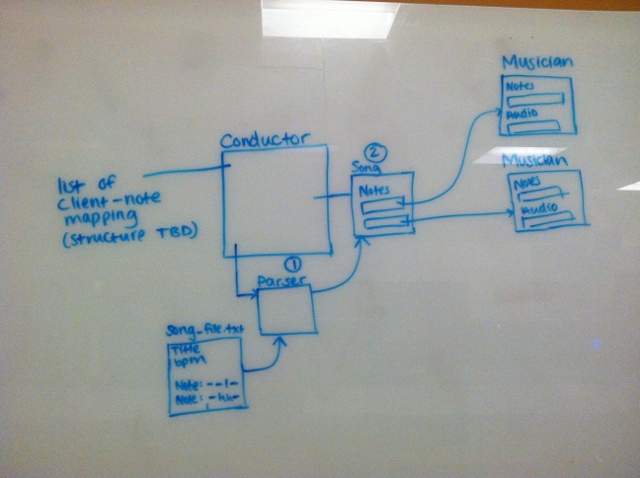
\includegraphics[width=\textwidth]{old_diagram}


% Analysis of Outcome
\section{Analysis and Reflection}

\subsection{Deliverable Status}
Our orchestra can play any song provided in the format described earlier in this report. Any machine
with PortAudio and PyAudio can join as a musician. The conductor does not need to have these
packages installed. We also accomplished an extra stretch goal of having the musician's terminal
light up when it is playing a note.

\subsection{Best Decision}
There were many design decisions that shaped our project, but the best decision we made was to
create a separate parsing module. Having the conductor call the module with the given song allows
us to parse the song however we choose. This modularity gives us the flexibility to change the
song format in the future, and it allowed us to accomplish our stretch goals of playing sharps and
flats as well as notes in multiple octaves without redesigning our entire project.

\subsection{Worst Decision}
The worst decision we made was to connect to the sound card every time a note was played.
Connecting to and disconnecting from the sound card causes a horrid clicking noise, ruining the
fluidity of the song. Changing this, however, would require a significant redesign of our musician.
This may have been caused by our decision to use PyAudio to play a sine wave, which stopped abruptly
after the specified duration ended. It does not resemble musical instruments, which gradually get
softer as the note finishes.


% Abstractions and Language
\section{Abstractions and Language} We have three major abstractions:

\begin{itemize}
\item The "conductor," or the server with which the musicians communicate.
\item The "musician," or a client which is given a note to play.
\item The parser, which takes a text-based representation of a song and converts it into a set of
frequencies, each of which has a list of starting times and durations, that the conductor can
distribute to musicians.
\end{itemize}

The implementation also contains an audio module. This module could be extended to attempt several
different methods of playing sound based on what packages are available on the client machine. At
present, the module either plays sound using PyAudio or does not play sound at all.


% Implementation Timeline
\section{Implementation Strategy}

\subsection{Timeline}
\begin{itemize}[parsep=0pt]
\item November 10:
    \begin{itemize}
    \item Had a working connection between conductor and musicians
    \item Handled new musicians and dropped connections
    \item Generated test files in parsable format
    \item Parsed input file through the conductor and sent sets of notes to musicians
    \end{itemize}
\item November 17:
    \begin{itemize}
    \item Gained access to Halligan 105 for testing
    \item Requested that packages be installed on Linux machines and Mac lab machines
    \item Began writing PyAudio-based play function
    \end{itemize}
\item November 24:
    \begin{itemize}
    \item Abandoned attempts to prevent the sound card of clicking
    \item Musicians could play their specified note
    \end{itemize}
\item December 1:
    \begin{itemize}
    \item Enforced consistent sense of timing among machines
    \item Had musicians attempt to reconnect to conductor when a connection is lost
    \item Lit up terminal screen when musician is actively playing
    \end{itemize}
% TODO re-add if we finish these things
\item December 5:
    \begin{itemize}
    \item Had musicians exit gracefully if they lose their connection to the conductor
%    \item Allowed conductor to be started with a list of songs so that the musicians can play a
%    concert
    \end{itemize}
\end{itemize}

\subsection{Reflection on Division of Labor}
We originally planned to work on all aspects of this project as a group. However, scheduling issues
prevented this from happening in several cases. As a result, not all group members were present for
certain design changes. More clearly defining who was responsible for which portions of the
implementation may have resulted in a more refined finished product.

% Bug Report
\section{Bug Report}
% TODO

% Code Overview
\section{Code Overview}
Our code is available on \href{https://github.com/TylerLubeck/ConcurrentMusic}{GitHub}. An
explanation of the program structure follows.

\subsection{Python Modules}
\begin{description}
\item[\texttt{audio.py}] Contains an audio class which constructs a function with which to play
sound, based on packages available on the musician.
\item[\texttt{conductor.py}] Contains the implementation of the conductor.
\item[\texttt{musician.py}] Contains the implementation of the musician.
\item[\texttt{note\_to\_freq.py}] Contains logic to convert from a letter note (such as C4 or A\#5)
to a frequency. Also contains logic to calculate the duration of a note based on the BPM of the
song.
\item[\texttt{parse.py}] Contains logic to concurrently parse a given song file.
\item[\texttt{suppress\_errors.py}] Contains handlers necessary to avoid printing excessive output
when PyAudio encounters errors.
\end{description}

\subsection{Other Files}
\begin{description}
\item[\texttt{songs/*}] A collection of songs in the correct format.
\item[\texttt{note.txt}] An ASCII note that can be displayed when a musician plays.
\item[\texttt{requirements.txt}] A list of necessary packages that can be installed via
\href{https://pypi.python.org/pypi/pip}{pip}.
\end{description}

\subsection{How To Run}
\begin{enumerate}
\item Install \href{http://www.portaudio.com/}{PortAudio} for your machine's architecture.
\item Install \href{http://people.csail.mit.edu/hubert/pyaudio/}{PyAudio}.
\item Clone the code from \href{https://github.com/TylerLubeck/ConcurrentMusic}{GitHub}.
\item Install other Python packages:\\
\texttt{pip install -r ConcurrentMusic/requirements.txt}
\item To start a conductor:\\
\texttt{python conductor.py --song <path to song> --port <port>}\\
The port number is optional and defaults to 8123.
\item To start a musician:\\
\texttt{python musician.py --ip <IP of conductor> --port <port of conductor>}\\
The port number is again optional and also defaults to 8123.
\end{enumerate}

\end{document}
